\section{Bases de datos sintéticas}
En la primera parte de la práctica utilizaremos una serie de experimentos sobre bases de datos sintéticas, que nos ayudarán a entender cómo funcionan las SVM y qué efectos producen sobre los resultados los dos parámetros que hay que especificar para entrenarlas.

\subsection{Trabajando con el primer dataset, pregunta 1, 2 y 3}

Este script comienza importando las librerías necesarias como es normal, en este caso numpy, matplotlib, pandas y sklearn para el acceso a SVM.
A continuación lee el CSV.

Podemos comprobar como el kernel que se utiliza es `lineal' y el parámetro C=1000.

\begin{figure}[H]
    \centering
    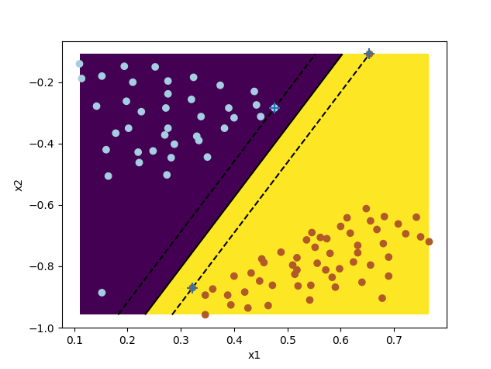
\includegraphics[scale=1.2]{img/dataset1}
    \caption{Dataset1, kernel lineal}
    \label{fig:Dataset1}
\end{figure}

En la Figura \ref{fig:Dataset1} tenemos las clases separadas mediante un hiperplano separador lineal.


La siguiente figura\ref{fig:Dataset1_1} corresponde solo a la nube de puntos del dataset1, es evidente que la manera más fácil de separar las clases es mediante un recta.
\begin{figure}[H]
    \centering
    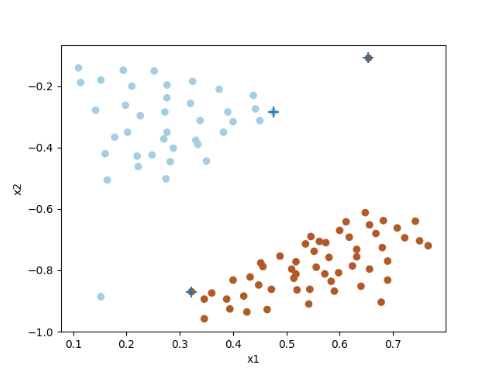
\includegraphics[scale=1.2]{img/dataset1_1}
    \caption{Nube de puntos dataset1}
    \label{fig:Dataset1_1}
\end{figure}

A continuación vamos a modificar el valor del parámetro C, podemos consultar su utilidad en \url{https://scikit-learn.org/stable/modules/generated/sklearn.svm.SVC.html}, el parámetro C es utilizado como regulador, define la penalización de que e cometan errores en la clasificación, la regularización es inversamente proporcional a C, un valor muy alto de C conllevará a un SVM que cometa el mínimo número de errores. Un valor de C pequeño por el contrario conllevará a un clasificador con el máximo margen, aunque se cometan errores en la clasificación. Por supuesto está relacionado con el posible sobre-entrenamiento.

%\begin{table}[H]
    %\centering
    %\small
    %\begin{tabular}{|c|c|}
    %    \textbf{C} & \textbf{CCR}\\ \hline
        
    %\end{tabular}
    %\caption{Dataset1, distintos valores de C}
    %\label{valoresC}
%\end{table}

\begin{figure}[H]
	\begin{subfigure}{0.48\textwidth}
    	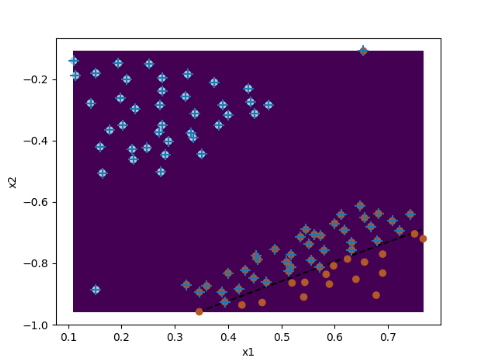
\includegraphics[width=\linewidth, height=1\linewidth]{img/10_-2}	
    	\caption{$C = 10^{-2}$}
	\end{subfigure}
	\hfill
	\begin{subfigure}{0.48\textwidth}
    	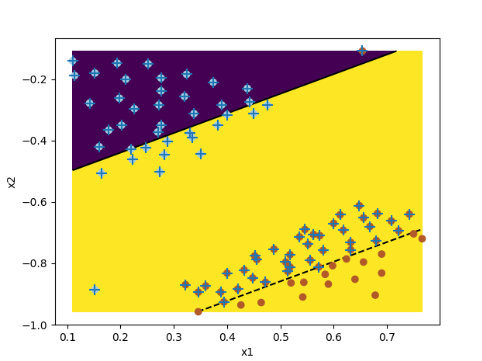
\includegraphics[width=\linewidth, height=1\linewidth]{img/10_-1}	
    	\caption{$C = 10^{-1}$}
	\end{subfigure}
	\begin{subfigure}{0.48\textwidth}
    	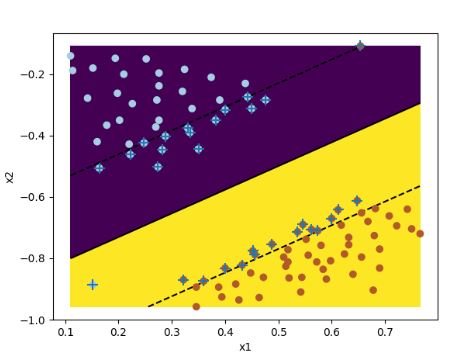
\includegraphics[width=\linewidth, height=1\linewidth]{img/10_0}	
    	\caption{$C = 10^{0}$}
	\end{subfigure}
	\begin{subfigure}{0.48\textwidth}
    	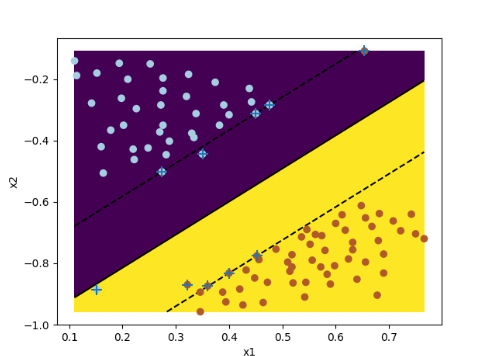
\includegraphics[width=\linewidth, height=1\linewidth]{img/10_1}	
    	\caption{$C = 10^{1}$}
	\end{subfigure}
	\begin{subfigure}{0.48\textwidth}
    	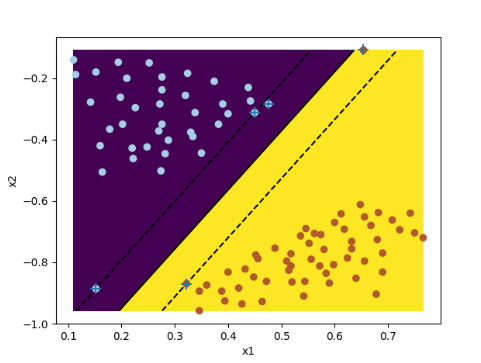
\includegraphics[width=\linewidth, height=1\linewidth]{img/10_2}	
    	\caption{$C = 10^{2}$}
	\end{subfigure}
	\begin{subfigure}{0.48\textwidth}
    	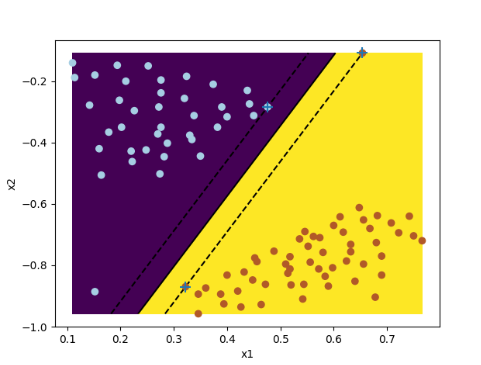
\includegraphics[width=\linewidth, height=1\linewidth]{img/10_3}	
    	\caption{$C = 10^{3}$}
	\end{subfigure}
	\caption{Variaciones del parámetro C}
	\label{fig:var1}
\end{figure}
	
\begin{figure}
	\centering
    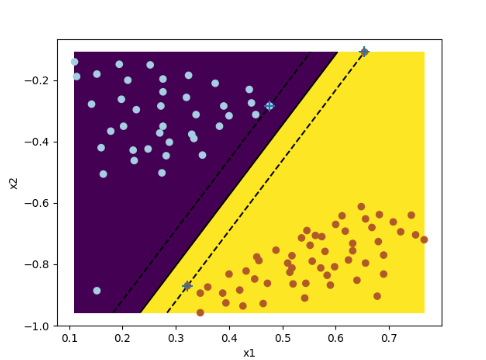
\includegraphics[scale=0.8]{img/10_4}	
    \caption{$C = 10^{4}$}
	\label{fig:var2}
\end{figure}

\subsection{Trabajando con el segundo dataset, preguntas 4 y 5}

\begin{figure}[H]
	\centering
	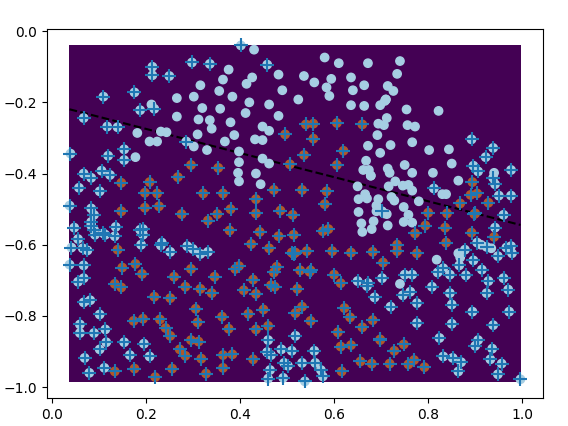
\includegraphics[scale=1]{img/dataset2_1}
    \caption{Dataset2 SVM lineal y $C=1000$}
    \label{dataset2}
\end{figure}

La figura\ref{dataset2} representa al segundo dataset con una SVM lineal y un parámetro $C=1000$, en ella podemos comprobar como es imposible separar las clases mediante una línea, por mucho que modifiquemos el parámetro C. \\
Mediante el uso de funciones de kernel tipo RBF podemos conseguir trabajar con este dataset, este kernel necesita un parámetro gamma que iremos introduciendo hasta encontrar una buena solución. En libsvm $\gamma = 1/2*radio^2$, para un radio alto tiende a soluciones más suaves, con menor sobre-entrenamiento, mientras que para un radio pequeño tiende a producir mas sobre-entrenamiento.

\begin{figure}[H]
	\centering
	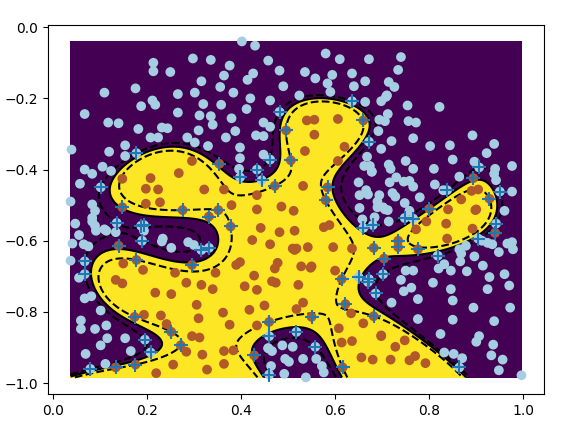
\includegraphics[scale=1]{img/dataset2_2}
    \caption{Dataset2 RBF, $C=1000$ $\gamma=13$}
    \label{dataset2_2}
\end{figure}

\begin{figure}[H]
	\begin{subfigure}{0.48\textwidth}
    	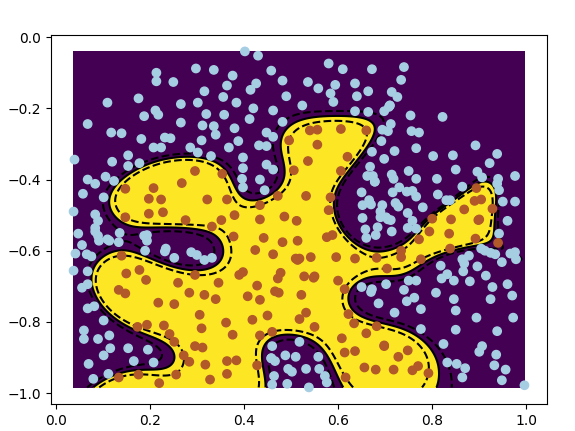
\includegraphics[width=\linewidth, height=1\linewidth]{img/dataset2_4}	
    	\caption{$C=1000$ $\gamma=50$}
	\end{subfigure}
	\begin{subfigure}{0.48\textwidth}
    	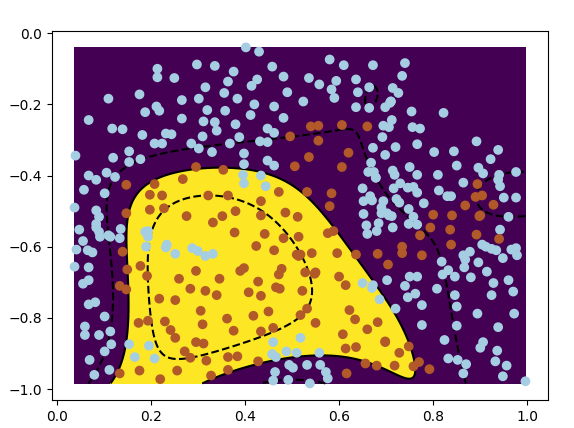
\includegraphics[width=\linewidth, height=1\linewidth]{img/dataset2_3}	
    	\caption{$C=1000$ $\gamma=2$}
	\end{subfigure}
	\caption{Sobreentrenamiento e infraentrenamiento}
	\label{sobreentrenamiento_infraentrenamiento}
\end{figure}

\subsection{Tercer dataset, preguntas de la 6 a la 11}

\begin{figure}[H]
	\centering
	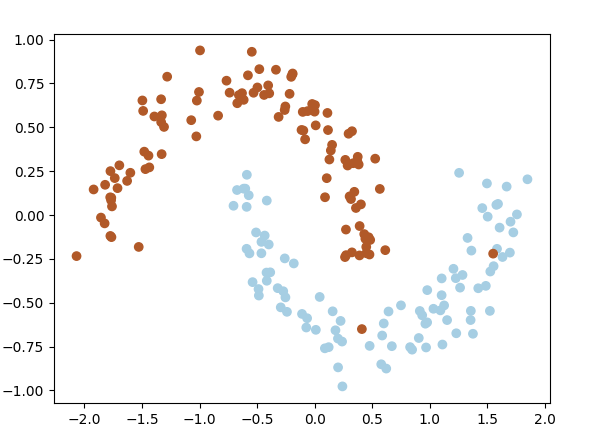
\includegraphics[scale=0.85]{img/dataset3_1}
    \caption{Dataset3 RBF, $C=1000$ $\gamma=1$}
    \label{dataset3_1}
\end{figure}

Comprobamos Fig\ref{dataset3_1} que este dataset tampoco es linealmente separable, volvemos a utilizar un kernel de tipo RBF. Hay un par de puntos que se salen de la densidad de la clase y se introducen en la otra, podríamos pensar que se tratan de outliers.

\begin{figure}[H]
	\centering
	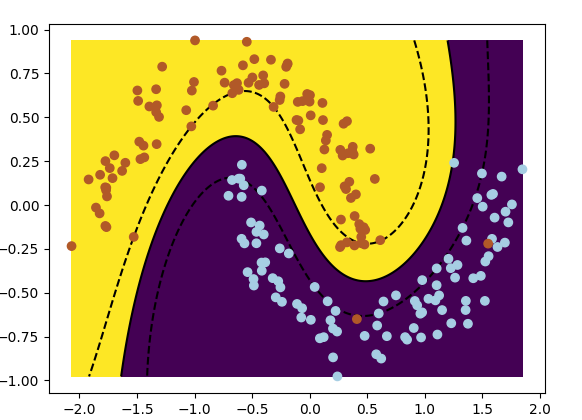
\includegraphics[scale=0.85]{img/dataset3_2}
    \caption{Dataset3 bien clasificado, RBF, $C=10$ $\gamma=1$}
    \label{dataset3_2}
\end{figure}

\begin{figure}[H]
	\begin{subfigure}{0.48\textwidth}
    	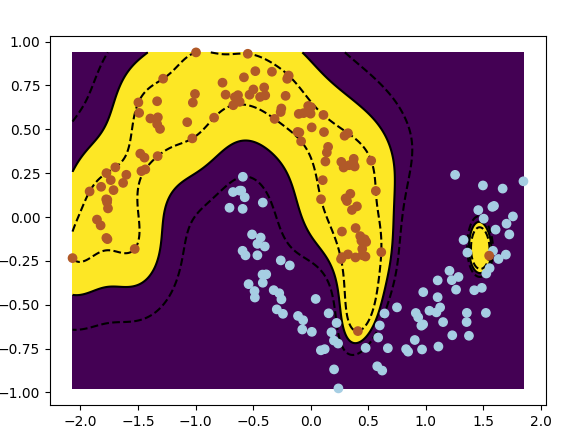
\includegraphics[width=\linewidth, height=1\linewidth]{img/dataset3_3}	
    	\caption{$C=1000$ $\gamma=10$}
	\end{subfigure}
	\begin{subfigure}{0.48\textwidth}
    	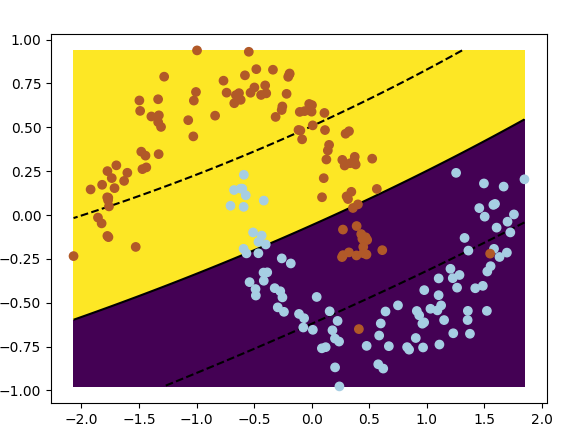
\includegraphics[width=\linewidth, height=1\linewidth]{img/dataset3_4}	
    	\caption{$C=10$ $\gamma=0.1$}
	\end{subfigure}
	\caption{Sobre-entrenamiento e infra-entrenamiento}
	\label{3_sobreentrenamiento_infraentrenamiento}
\end{figure}

\subsection{Base de datos noMNIST}
Esta base de datos está formada por 900 patrones de entrenamiento y 300 patrones de test. Está formada por un conjunto de letras (de la a hasta la f), están ajustadas a una rejilla cuadrada de 28 x 28 píxeles.

El proceso de validación cruzada se repite completo para todas las combinaciones posibles de parámetros C y $\gamma$, en este caso $ 7X7X5 = 245$. Obteniendo un CCR de 81,77 \%.

A continuación en la tabla \ref{k_fold} indicamos el CCR obtenido junto con su tiempo para distintos tamaños de k-fold.
\begin{table}[H]
\centering
	\begin{tabular}{|c|c|c|}
	\hline 
	K & CCR & Tiempo \\ 
	\hline 
	3 & 82,22\% & 11.4 s \\ 
	\hline 
	5 & 81,77\% & 25.01 s \\ 
	\hline 
	10 & 81,77\% & 66.42 s \\
	\hline
	\end{tabular}
	\caption{Resultados validación cruzada K-fold}
	\label{k_fold}
\end{table}

Comprobamos como el mejor resultado ha sido para $K = 3$, además también se consigue con menos tiempo.


\subsection{Base de datos Clasificación de SPAM}
Uno de los campos donde se utiliza el aprendizaje automático con un mayor éxito es la detección automática de spam en servidores de correo. El fichero de entrenamiento contiene 4000 correos, mientras que el de test tiene 1000 correos. Ambos utilizan la lista de vocabulario de 1899 palabras contenida en vocab.txt. Por tanto, cada patrón tiene 1899 valores binarios.

Entrenaremos un modelo lineal de SVM con distintos valores de C.
\begin{table}[H]
\centering
	\begin{tabular}{|c|c|}
	\hline 
	C & CCR \\ 
	\hline 
	0.01 & 98\% \\ 
	\hline 
	0.1 & 98.9\% \\ 
	\hline 
	1 & 97.8\% \\
	\hline
	10 & 97.5\% \\
	\hline
	\end{tabular}
	\caption{Resultados bases datos SPAM}
	\label{k_fold}
\end{table}